%%%%%%%%%%%%%%%%%%%%%%%%%%%%%%%%%%%%%%%%%%%%%%%%%%%%%%%%%%%%%%%%%%%%%%


%%% Preamble
\documentclass[paper=a4, fontsize=11pt]{scrartcl}
\usepackage[T1]{fontenc}
\usepackage{fourier}

\usepackage[english]{babel}															% English language/hyphenation
\usepackage[protrusion=true,expansion=true]{microtype}	
\usepackage{amsmath,amsfonts,amsthm} % Math packages
\usepackage[pdftex]{graphicx}	
\usepackage{url}

%% BEGIN ADDED FOR FAQ Section
\usepackage[margin=1in]{geometry} % Required to make the margins smaller to fit more content on each page
\usepackage[linkcolor=blue]{hyperref} % Required to create hyperlinks to questions from elsewhere in the document
\hypersetup{pdfborder={0 0 0}, colorlinks=true, urlcolor=blue} % Specify a color for hyperlinks
\usepackage{todonotes} % Required for the boxes that questions appear in
\usepackage{tocloft} % Required to give customize the table of contents to display questions
\usepackage{microtype} % Slightly tweak font spacing for aesthetics

% Create the command used for questions
\newcommand{\question}[1] % This is what you will use to create a new question
{
\refstepcounter{questions} % Increases the questions counter, this can be referenced anywhere with \thequestions
\par\noindent % Creates a new unindented paragraph
\phantomsection % Needed for hyperref compatibility with the \addcontensline command
\addcontentsline{faq}{questions}{#1} % Adds the question to the list of questions
\todo[inline, color=gray!10]{\textbf{#1}} % Uses the todonotes package to create a fancy box to put the question
\vspace{1em} % White space after the question before the start of the answer
}
%% END QUESTION ADD

% Algorithms package
\usepackage{fancybox}
\usepackage{algorithm}
\usepackage{caption}
\usepackage{algorithmic}



%%% Custom sectioning
\usepackage{sectsty}
\allsectionsfont{\centering \normalfont\scshape}


%%% Custom headers/footers (fancyhdr package)
\usepackage{fancyhdr}
\pagestyle{fancyplain}
\fancyhead{}											% No page header
\fancyfoot[L]{}											% Empty 
\fancyfoot[C]{}											% Empty
\fancyfoot[R]{\thepage}									% Pagenumbering
\renewcommand{\headrulewidth}{0pt}			% Remove header underlines
\renewcommand{\footrulewidth}{0pt}				% Remove footer underlines
\setlength{\headheight}{13.6pt}


%%% Equation and float numbering
\numberwithin{equation}{section}		% Equationnumbering: section.eq#
\numberwithin{figure}{section}			% Figurenumbering: section.fig#
\numberwithin{table}{section}				% Tablenumbering: section.tab#


%%% Maketitle metadata
\newcommand{\horrule}[1]{\rule{\linewidth}{#1}} 	% Horizontal rule

\title{
		%\vspace{-1in} 	
		\usefont{OT1}{bch}{b}{n}
		\normalfont \normalsize \textsc{PacBio Variant Calling Group} \\ [25pt]
		\horrule{0.5pt} \\[0.4cm]
		\huge The ConsensusCore Scoring Model \\
		\horrule{2pt} \\[0.5cm]
}
\author{
		\normalfont 								\normalsize
        Nigel Delaney\\[-3pt]		\normalsize
        \today
}
\date{}


%%% Begin document
\begin{document}
\maketitle
\section{Introduction}

The ConsensusCore scoring model calculates the score that a read comes from a particular template.  It calculates this for a given template and a read using information from the reads associated QV and Tag values.  The scoring algorithm implements dynamic programming to find the score either through all paths, or through the single best path.  This algorithm is similar to standard dynamic programming routines, with some modifications described here. \footnote{If you are not familiar with these techniques, none of this will make sense.  The standard introduction to this material is the first 4 chapters of "Biological Sequence Analysis" by Durbin, Eddy, Krogh and Mitchison.}

Each position in the read is associated with several QV values that affect the score, however these values are not used directly or interpreted as probabilities.  Prior to computing the score, each QV value undergoes an affine transformation using parameters specific to that chemistry and derived by a training step.  In the case of MergeQV values, this transformation is distinct for each of the 4 possible bases. Similarly, the InsertionQV values are transformed in one of two ways depending on the relationship between the read base and the template as described below.
 




\section{ Scoring Procedure} 

The inputs are a read of length, I, and a template of length J.  Each base in the read also has an associated value for InsertionQV, SubstitutionQV, MergeQV, DeletionQV and DeletionTag.  The algorithm proceeds by recursively populating a matrix and returning the bottom right value as described next.\footnote{This section derived from the code in \texttt{QvEvaluator.cpp} and \texttt{SimpleRecursor.cpp}.}  In describing the algorithm and to account for offsetting, in what follows read and template positions are 1-based indexed, while positions in the matrix that are filled are referred to by 0-based indexes. Currently, the scoring algorithm populates the matrix using the maximum value of the possible moves, but equivalently it could use the summation.




\begin{algorithm}
\caption*{\textbf{Score Calculation Algorithm}}
\label{calcScore}
\begin{algorithmic}[h]
\FOR{$j=1$ to J}
\FOR{$i=1$ to I}
\IF{ $i =0\ \& j =0 $}
\STATE $A[i,j] = 0$
\ELSIF {$i =0 \text{ or } j =0$}
\STATE $A[i,j] = -\infty $
\ELSE
\STATE \[
	A[i,j]  \leftarrow \text{max}
\begin{cases}
\text{Match Score} \\
\text{Insertion Score} \\
	\text{Deletion Score} \\
   		\text{Merge Score} \end{cases}
\]
\ENDIF	
\ENDFOR
\ENDFOR
\RETURN $A[I,J]$
\end{algorithmic}
\end{algorithm}


\subsection*{Recursion}



\section{Scoring Steps in the Dynamic Programming Recursion}
After the matrix is initialized, each element in the matrix is recursively populated by examining the available moves, either an insertion, deletion, match or merge.  If a particular step cannot be calculated because it is too close to the edge, it is skipped.  Each possible move is described next, and figure~\ref{fig:everything} shows the initial conditions as well as all positions in the matrix, read and template that are evaluated in order to calculate the value for a given score.


\begin{figure}[H] %% The [h] means place the figure about here.
	\includegraphics{Everything}
		\caption{\textbf{Initial Conditions and Needed Information:} The information required for calculating the score for the matrix position denoted by the blue box.  Red boxes indicate values that must already be calculated, and colored bases indicate positions in the read and the template that are evaluated to determine the score.  The first row and column have also been filled with their initial values.}		
		\label{fig:everything}		
\end{figure}




\subsection{\textbf{Match Score}}

\begin{figure}[H] %% The [h] means place the figure about here.
	\includegraphics{Match}
		\caption{The calculation of the match score.  The upper element is added to an amount determined by the comparison of the bases shown.}
\end{figure}
\[
	\text{Match Score} = \alpha_{i-1,j-1}  +  \begin{cases}
							 \ \text{A fixed value} & \text{if }  R_{i} = T_{j} \\
							 \text{Substitution score given for } R_{i} & \text{if }  R_{i}  \neq T_{j} 
							 \end{cases}
\]

This is the standard match score, but the score given matching bases is not affected by the Substituion score for that base.  


\subsection{\textbf{Insertion Score}}

\begin{figure}[H] %% The [h] means place the figure here.
	\includegraphics{Insertion}
		\caption{The calculation of the insertion value.  The upper diagonal element is added to an amount determined by the comparison of the bases shown.}
\end{figure}

\[
	\text{Insertion Score} = \alpha_{i-1,j}  +  \begin{cases}
							 \text{Insertion score  for } R_{i} \text{ scaled to a branch step} & \text{if }  R_{i} = T_{j+1} \\
							 \text{Insertion score  for } R_{i} \text{ scaled to a non-branch step} & \text{if }  R_{i}  \neq T_{j+1} 
							 \end{cases}
\]


The insertion score differs from typical insertion scoring due to the "branching" process that occurs during nucleotide incorporation.  The polymerase may begin to incorporate a base and hold it long enough for the base to be detected in the sequencer before eventually releasing it after failing to complete the incorporation reaction.  In the event of a true branch, the inserted base should thus match the next template base.  This rule is a slight approximation because in certain edge cases (e.g. local alignments that never match the next base, or windowed areas that exclude the next base) it is not entirely accurate to say whether a branch did or did not occur.

The insertion score for the read base is used differently depending on whether or not it is a branch step.  If a branch, it is scaled by one affine transformation, and if not a branch it is scaled by another.




\subsection{\textbf{Deletion Score}}

\begin{figure}[H] %% The [h] means place the figure about here.
	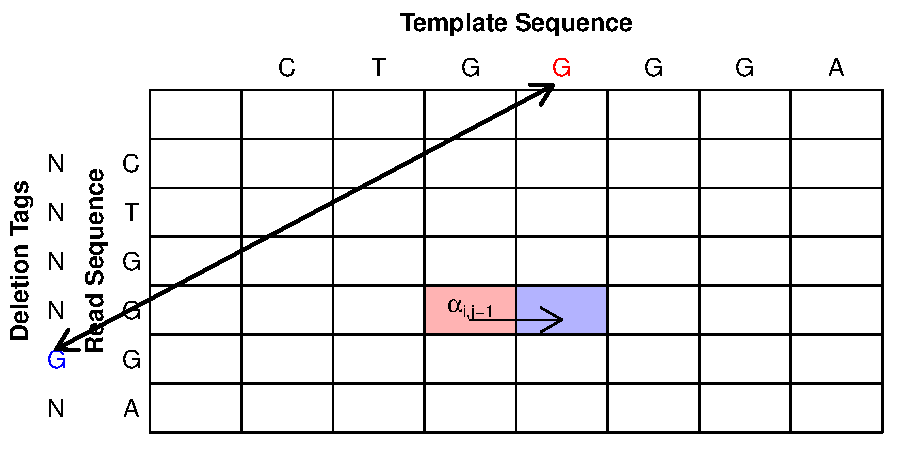
\includegraphics{Deletion}
		\caption{The calculation of the deletion score.  The left matrix element is added to an amount determined by the comparison of the bases shown.}				
\end{figure}

\[
	\text{Deletion Score} = \alpha_{i,j-1}  +  \begin{cases}
							 \text{Deletion score  for } R_{i+1}  & \text{if }  \text{DeletionTag}_{i+1} = T_{j} \\
							 \text{A fixed constant} & \text{if }  \text{DeletionTag}_{i+1} \neq T_{j} 
							 \end{cases}
\]

The deletion score also differs from what is typical.  A small subset of bases in HQ regions (\textasciitilde10\%) contain a DeletionTag base that is not equal to N.  This base reports the most likely base that was deleted immediately before that base.  If a position in the template is deleted, the score changes if it matches the next positions most likely deleted base.




\subsection{\textbf{Merge Score}}
\begin{figure}[H] %% The [h] means place the figure about here.
	\includegraphics{Merge}
		\caption{The calculation of the merge.  The upper left "knight's move" matrix element is added to an amount determined by the comparison of the bases shown.}				
\end{figure}

\[
	\text{Merge Score} = \alpha_{i-1,j-2}  +  \begin{cases}
							 \text{Merge score based on nucleotide in } R_{i}  & \text{if }  R_{i} = T_{j} \text{ \& } R_{i} = T_{j-1} \\
							 \text{A fixed constant (typically }-\infty\text{)} & \text{otherwise}
							 \end{cases}
\]

The merge score is the most unusual aspect of this recursion relative to standard methods.  It is designed to account for the possibility that two bases were read simultaneously as one base (presumably because the enzyme acquired the next base before a break in the signal intensity was observed, and if this was the same base, this could be interpreted as one merged pulse).

From an alignment perspective, this move is equivalent to a deletion followed by a match, but scored with a different penalty.  Combined with the other novelties in PacBio scoring, this makes the scoring of regions with homopolymers more complicated than in typical models.  For example, consider the alignment:

\begin{center}
\texttt{GGGG}

\texttt{GG-G}
\end{center}

The deletion in this alignment can be explained by either a single merge move or a deletion move followed by a match.  Because deletions can be scored in one of two ways depending on the deletion tag values, this creates three separate possible scorings for the single deletion.  Based on typical values for QV scores, if there is a DeletionTag matching the deleted base is available, the path with the deletion followed by match is preferred.  If not, then a merge is typically employed over a deletion and a match, provided the merge value is above the dotted blue line shown in figure ~\ref{fig:violin}.

\newpage

\newlistof{questions}{faq}{\large } % This creates a new table of contents-like environment that will output a file with extension .faq
\setlength\cftbeforefaqtitleskip{4em} % Adjusts the vertical space between the title and subtitle
\setlength\cftafterfaqtitleskip{1em} % Adjusts the vertical space between the subtitle and the first question
\setlength\cftparskip{.3em} % Adjusts the vertical space between questions in the list of questions

%----------------------------------------------------------------------------------------
%	TITLE AND LIST OF QUESTIONS
%----------------------------------------------------------------------------------------

\begin{center}
\Huge{\bf \emph{Common Questions}} % Main title
\end{center}
\listofquestions % This prints the subtitle and a list of all of your questions


%----------------------------------------------------------------------------------------
%	QUESTIONS AND ANSWERS
%----------------------------------------------------------------------------------------

\question{What information from a read is used to calculate a score given a template?}\label{new-question}

All the features in QvSequenceFeatures class (\texttt{Features.hpp)}

\begin{itemize}
	\item BaseCalls
	\item DeletionQV 
	\item DeletionTag
	\item SubsQV
	\item InsQV
	\item MergeQV
\end{itemize}	


%------------------------------------------------

\question{Will the reverse complement of a read/template give the same score?}\label{labels}

\textbf{No}.  Because the affine transformation of QV scores is specific to the type of base (A, C, G or T), strand matters.  This reflects the biological reality of the enzyme.

\question{When is a MergeQV assigned a value of 100?}\label{merge100}

If when merging pulses into calls a segment less than 3 frames wide is encountered, a merge is considered impossible and a zero probability of error is returned.  This 0 is then converted to a QV value that is automatically capped at QV = 100.

\question{What are the typical ranges of the different QV values?}

The violin plot below shows a sampling of P6-C4 QV scores from different ZMWs in the HQ region. The plot has been made after transforming the QV values into their actual scores using the affine recalibration implemented for CCS.  Only DeletionQV values when the DeletionTag was not an 'N' are shown.

\begin{figure}[h] %% The [h] means place the figure about here.
	\includegraphics{qv_violin_p6c4}
		\caption{Violin plot of QV scores.  The horizontal lines represent fixed scoring constants, with blue being the deletion penalty, and red the match score.  The dotted blue line is the sum of the constant deletion and match penalties. The SubsQV violin plot has been rescaled in order to be visible, as approximately 95\% of all values are the lowest value shown, which makes it impossible to see the others.}	
		\label{fig:violin}			
\end{figure}


%%% End document
\end{document}